\documentclass[sigconf,review,anonymous]{article}
% if you need to pass options to natbib, use, e.g.:
%     \PassOptionsToPackage{numbers, compress}{natbib}
% before loading neurips_2020

% ready for submission
%\usepackage{neurips_2020}

% to compile a preprint version, e.g., for submission to arXiv, add add the
% [preprint] option:
%     \usepackage[preprint]{neurips_2020}

% to compile a camera-ready version, add the [final] option, e.g.:
     \usepackage[final]{neurips_2020}

% to avoid loading the natbib package, add option nonatbib:
     %\usepackage[nonatbib]{neurips_2020}
\usepackage{multirow}
\usepackage[table,xcdraw]{xcolor}
\usepackage[utf8]{inputenc} % allow utf-8 input
\usepackage[T1]{fontenc}    % use 8-bit T1 fonts
% \usepackage{hyperref}       % hyperlinks
% \usepackage{url}            % simple URL typesetting
\usepackage{booktabs}       % professional-quality tables
\usepackage{amsfonts}       % blackboard math symbols
\usepackage{nicefrac}       % compact symbols for 1/2, etc.
\usepackage{microtype}      % microtypography
\usepackage{float} % here for H placement parameter
% \usepackage{multirow}
% \usepackage[normalem]{ulem}
% \useunder{\uline}{\ul}{}
% \usepackage{xcolor}
\usepackage[table,xcdraw]{xcolor}
\usepackage[obeyspaces]{url}
\usepackage{graphicx}
\usepackage{listings}
\usepackage{enumerate}
\usepackage{amsmath}
\definecolor{codegreen}{rgb}{0,0.6,0}
\definecolor{codegray}{rgb}{0.5,0.5,0.5}
\definecolor{codepurple}{rgb}{0.58,0,0.82}
\definecolor{backcolour}{rgb}{0.95,0.95,0.92}



\lstset{style=mystyle}
\usepackage{algorithm}
\usepackage[noend]{algpseudocode}

\makeatletter
% Reinsert missing \algbackskip
\def\algbackskip{\hskip-\ALG@thistlm}
\makeatother


\title{Realizing Literate Programming using Neural Machine Translation}

% The \author macro works with any number of authors. There are two commands
% used to separate the names and addresses of multiple authors: \And and \AND.
%
% Using \And between authors leaves it to LaTeX to determine where to break the
% lines. Using \AND forces a line break at that point. So, if LaTeX puts 3 of 4
% authors names on the first line, and the last on the second line, try using
% \AND instead of \And before the third author name.
\author{%
  Anonymous Author(s)
}
% \author{%
  
%   Hung Phan \\
%   Department of Computer Science \\
%   Iowa State University\\
%   Ames, IA 50011 \\
%   hungphd@iastate.edu \\
% }

\begin{document}

\maketitle

\begin{abstract}

Literate Programming (LP) is a programming paradigm that unites natural language (NL) with code as one document, which helps the developer to explain the logic of some parts of the code using a natural language. 
However, despite having advantages for code understanding,  LP hasn't been applied in practice mainly because there is no tool to automatically generate a correct and compilable code, and developers are required to manually specify the code for the natural language description which is a tedious and error-prone process. 
In this paper, we provide a context-aware tool called InvocMap to realize LP that allows developers for writing the description of methods inside the code environment and get the correct compilable Method Invocation (MI) code. 
Different from existing related works and other code suggestion tools such as AnyCode which only considered the given natural language description as input, we analyze the input from two different sources, i.e. NL description and its surrounding context. 
InvocMap proposes a semi-supervised approach based on three major modules. 
First, it uses unsupervised Neural Embedding to handle NL description of MIs to a list of possible method names. 
Contrary to expensive supervised machine learning methods that require a big dataset of the parallel corpus with NL and programming language.
Second, Machine Translation models trained from large scale code corpus to learn the structure of MIs, given a list of method names and surrounding code context. 
Third, a program analysis method that assigns local variables to structure of MIs to get the final code. 
InvocMap operates in two modes of input for describing MIs for developers, from method names directly, and from natural language description. 
By evaluation on data from 1000 high-quality Java projects, we got the accuracy as up to 90\% for MI suggestion from method names, and over 60\% for MI suggestion from NL description, which outperforms the prior works and shows the potential of our approach for realizing LP.


%Literate Programming (LP) is a programming paradigm that unites natural language with code as one document, which helps the developer to explain the logic of some parts of the code in a natural language. However, despite having advantages for code understanding,  LP hasn't been extensively applied in practice mainly because of two reasons. First, developers are required to specify the code for each natural language description manually which is a tedious and error-prone process. Secondly, supervised machine learning approaches for automatically retrieving code from Natural Language is expensive since it required a big dataset of the parallel corpus with NL and Programming Language. In this paper, we provide a tool InvocMap to realize LP to allow developers for writing the textual description of Method Invocations (MIs) inside code environment and get the correct MIs. Different from other code suggestion tools as AnyCode which was only considered natural language as input, we analyze the input from 2 sources: the NL description and its surrounding context. InvocMap proposes a semi-supervised approach by 3 modules. First, it uses unsupervised Neural Embedding to handle NL description of MIs to a list of possible method names. Second, Machine Translation models are trained from large scale code corpus to learn the structure of MIs given a list of method names and surrounding code context. Third, a program analysis step is proposed to assign local variables to structure of MIs to get the final code. InvocMap provides 2 modes of input for describing MIs for developers: from method names directly and from natural language description. By evaluation with training data from 1000 Java high-quality projects, we got the accuracy as up to 90\% for MI suggestion from method names and over 60\% for MI suggestion from NL description, which is outperforming the prior work AnyCode and showing the potential of realizing LP which is specified for supporting NL descriptions of MIs.
\end{abstract}

\section{Introduction}
Literate Programming (LP), which was introduced by Donald E. Knuth \cite{001}, is intended to support software developers by a convenient programming environment. The idea of LP is to construct a sample program by an alternative way. The construction of program by LP is considered as a process contained two observations. First, they can consider the program as a list of statements which is handled by a compiler in programming language. This observation is traditional and be familiar with developers. The second observation is to consider a programming task as a description in the form of a natural language. Unlike the first observation, the second observation proposes a new way of program representation by literature. It helps the program not only runable but also explainable in human natural language. An application of LP is the WEB system \cite{001}, which can output the program as natural description and Pascal programming language by Tangle and Waive library. LP does not only provide advantages in better programming experiences, but also introduces a solution for education of how to programming, based on the appearance of documentation for each code snippets.
%Literate Programming (LP), which was invented by Donald E. Knuth \cite{001}, is intended to support software developers by a convenient programming environment. The idea of LP is to construct a sample program by an alternative way. The construction of program by LP is considered as a process contained two observations. First, they can consider the program as a list of statements which is handled by a compiler in programming language. This observation is traditional and be familiar with developers. The second observation is to consider a programming task as a description in the form of natural language. Unlike the first observation, the second observation proposes a new way of program representation by literature. It helps the program not only runnable but also explanable in human natural language. An application of LP is the WEB system \cite{001}, which can output the program as natural description and programming language in Pascal by Tangle and Waive library. LP does not only provide advantages in better programming experiences, but also introduce a solution for education of how to programming, based on the appearance of documentation for each code snippets.
\\
Despite having many advantages, the LP program paradigm has not been used popularly since its appearance in 1984. To the best of our knowledge, the most recent application which applied LP is done by Haghish et al \cite{005}, which provides support for visualizing LP in HTML format. The most well-known LP dataset \cite{006} provides a dataset of code in the form of combination between Natural Language (NL) and source code. \cite{004} studies about the problems which prevent LP to be practical. First, the number of developers who can be good both at programming and documenting their code are limited. In the other words, developers seem to be good only at the first observation than the second observation. Second, all of LP systems like \cite{006} require manually defining the source code related to each natural language description. The cost for manually representing the code by NL and programming language (PL) for every code snippets of large scale corpus is expensive. Thus, it is important to have a system that automatically derives the code from NL description in a code environment, to make LP feasible.
%Despite having many advantages, the LP program paradigm has not been used popularly since its appearance in 1984. Based on our knowledge, the most recent application which applied LP is provided by  Haghish et al \cite{005}, which provide support for visualizing LP in HTML format. The most well-known LP dataset is \cite{006}, which provides LP dataset of code which are in the form of combination between Natural Language (NL) and code. \cite{004} studies about the problems which prevent LP to be practical. First, the number of developers who can be good at programming and documenting their code are limited. In the other words, developers seems to be good only at the first observation than the second observation of LP. Secondly, all of LP system like \cite{006} require manually defining the source code related to each natural language description. The cost for manually representing the code by NL and programming language (PL) for every code snippets of large scale corpus is expensive. Thus, it is important to have a system that automatically deriving the code from NL description in a code environment, to make LP feasible.
\\
To the best of our knowledge, there is no work directly on generating code for natural language parts to support LP in Software Engineering (SE) and Machine Learning (ML). However, the problem of generating code from natural language (NL) is considered generally as one of the interesting research problems in SE. In related works, AnyCode \cite{007} provides a solution for synthesizing expression, mostly in the form of Method Invocations (MIs) by proposing the language model called Probabilistic Context Free Grammar (PCFG). Other works applied and optimized Machine Translation (MT) by providing supervised approaches for inferring code from natural description and vice versa. \cite{008} provides a tree based code generation which can be integrated in Recurrent Neural Network (RNN) for Python. \cite{009} applied Statistical Machine Translation (SMT) model for learning pseudo code from actual code for code summarization. This trend of research requires manually annotated data for supervised learning, which is expensive when applied in other types of NL. Although NL description and code can be extracted from large scale code repository, parallel corpus extracted by this way is usually erroneous and noisy.  Barone  et al. \cite{010} conduct a Python corpus by automatically extracting documentation and implementation of the same Python methods. By the experiment, they show that applying Machine Translation models to this corpus is challenging since the accuracy on both SMT and Neural Machine Translation (NMT) are low.
%From our knowledge, there is no tools or research projects which work directly on generating code for natural language parts for support LP in Software Engineering (SE) and Machine Learning (ML). However, the problem of generating code from natural language (NL) is one of interesting research problem in SE. In these works, AnyCode \cite{007} provides a solution for synthesizing expression, mostly in the form of Method Invocations (MIs) by proposing the language model called Probabilistic Context Free Grammar (PCFG). Other works applied and optimized Machine Translation (MT) by providing supervised approaches for inferring code from natural description and vice versa. \cite{008} provides a tree based code generation which can be integrated in Recurrent Neural Network (RNN) for Python. \cite{009} applied Statistical Machine Translation (SMT) model for learning pseudo code from actual code for code summarixation. This trend of research require manually annotated data for supervised learning, which is expensive when applied in other types of NL. Although NL description and code can be extracted from large scale code repository, parallel corpus extracted by this way is usually erroneous and contain noise.  Barone  et al. \cite{010} conduct a Python corpus by automatically extracting documentation and implementation of the same Python methods. By the experiment, they show that applying Machine Translation models to this corpus is challenging since the accuracy on both SMT and Neural Machine Translation (NMT) are low.
\\
All of existing works \cite{007,008,009,010} on generating code from natural language as input do not consider LP and were not designed to support LP. They treat solely the natural language as the entire input and provide the generated code as output, without considering a combination of code and NL text and neglecting the information from the surrounding code. \cite{010} considered the input as natural description of functions in Java Documentation (JavaDoc) for each functions of Python. AnyCode (\cite{007}) provides a solution for getting MIs by standalone NL queries instead of NL elements inside the code. In the other words, the expressions generated from AnyCode is consistent regardless the surrounding code and context.
%All of current works on generating code from natural language input like \cite{007,008,009,010} were not designed to support LP. They treat the natural language as the entire input and provide the output as generated code, without considering the information from surrounding code. \cite{010} considered the input as natural description of functions in Java Documentation (JavaDoc) for each functions of Python. AnyCode (\cite{007}) provides a solution for getting MIs by NL queries instead of NL element inside the code. In the other words, the output of expressions generated from AnyCode is consistent regardless the surrounding code.
\\
This paper is an attempt to realize Literate Programming by proposing InvocMap, a tool that helps developers to define natural language description of method invocations at any locations inside the code environment and automatically suggests MIs for all NL descriptions. Unlike prior works, we consider the input as an LP code snippet and consider code as a combination of sequence of code elements and natural language elements (NL-E). We provide the output as code snippet that all of NL-E were transformed to MIs. To achieve the solution, we provide a semi-supervised approach which combines three techniques: neural embedding to get method names from surrounding context and natural language elements; machine translation to get the parsed tree of MIs; program analysis techniques to analyze the surrounding context and instrument information to tree representation for getting the final code. In summary, We provide the following contributions:
\begin{itemize}
	\item Another viewpoint for considering natural language elements with information of surrounding code before and after it. 
	\item An approach for automatically generating method names based on all NL description and code information. 
	\item A Machine Translation model which converts text to tree data structure of Method Invocations.
	\item A code suggestion tool to realize LP by two modes: we allow developers to input method names and get method invocations, or  write free-form NL elements and get the suggested code.
\end{itemize}
%In this paper, we want to realizing Literate Programming by providing InvocMap, a tool that helps developers to define natural language description of method invocations at any locations inside the code environment and automatically suggesting MIs for all descriptions. Unlike prior works, we consider the input as a LP code snippet, which considers code as the combination of sequence of code elements and natural language elements (NL-E). We provide the output as code snippet that all of NL-E were transformed to MIs. To achieve the solution, we provide a semi-supervised approach which combines three techniques: neural embedding to get method names from surrounding context and natural language element; machine translation to get the parsed tree of MIs; Program Analysis to analyze the surrounding context to instrument information to tree to get the final code. We provide following contributions:
%\begin{itemize}
%	\item Provided another viewpoint for considering natural language element with information of code before and after it. 
%	\item Implemented an approach for automatically generating possible method names based on all NL and code information. 
%	\item Built a Machine Translation model which converted from text to tree data structure of Method Invocation.
%	\item Provided a code suggestion tool InvocMap to realizing LP by 2 modes. In the first mode, we allow developers to input method names and other information to get the method invocations. In the second mode, developers can write free form NL elements and get suggested code as list of MIs which the highest ranking suggested option as the most relevant code suggested by InvocMap.
%\end{itemize}

\section{Background}
In this part, we provide description for important terms and definitions we use for this research. Besides terms are well-known in Software Engineering, we define a set of terms which are used as elements in our approach.

\begin{enumerate}[\indent {}]
        \item \textbf{Abstract Syntax Tree (AST)} is a tree representation of tokens which are generated from statements and expressions in programming language (PL) \cite{011}.
        \item \textbf{Method Invocation (MI)} is one type of AST. MI can be described by combination of two elements: the parsed tree and local variables/literals which are usually located at the leaf level of the tree (terminals) \cite{012}. 
        \item \textbf{Structured AST (S-AST or SAST)} is the data structure that we defined in this paper. S-AST is the tree representation of MI but doesn't include information about name of local variables/literals. S-ASTs are extracted by visiting MIs in code corpus and abstracting local variables. An example of S-AST is shown in Figure \ref{figMotivatingExample}.
        \item \textbf{Core Method Name (C-MN)} is the name of MI which is appeared as the root node of S-AST. For example, in Figure \ref{figMotivatingExample}, the C-MN is \texttt{containsKey}. 
        \item \textbf{Literate Programming Code Snippet (LP-CS)} is a code snippet that contains one to multiple natural language description (element) for method invocations. LP-CS contains three following elements.
        \item \textbf{Natural Language Element (NL-E), PreCode, PostCode}: NL-E is the description in NL. \textbf{PreCode} of NL-E is the list of code tokens appeared before NL-E. \textbf{PostCode} is the list of code tokens appeared after NL-E. Example of NL-E is shown in Figure \ref{figMotivatingExample}.
        
        \item \textbf{Variables and Terms of NL-E}: Variables of NL-E are all tokens related to string and numeric literal along with variables defined in NL-E. Terms of NL-E are tokens of NL-E which are not in list of variables. 
    \end{enumerate}




\section{The \textit{InvocMap} Model}
\subsection{Problem Formulation}
InvocMap works as a semi-supervised translation engine. It relies on 2 viewpoints. First, we take advantages of all information of LP-CS including the natural language part and surrounding code. Second, we learn the transformation from the abstract level of method invocations as C-MN to the structured tree representation in high quality large scale code corpus. 
\\
The code suggestion by InvocMap is provided by the process illustrated in Figure \ref{figOverview}. First, given input as code snippet with natural language, the Tokenization will extract all tokens related to both NL,PreCode and PostCode. Our approach solves input of all Machine Learning models in the form of words/tokens. Next, an unsupervised approach is provided by Doc2Vec \cite{002} to learn 2 contexts of each C-MN in large scale code corpus as PreCode and PostCode of them to the list of C-MNs which have closest context in vector representation to given NL-E. Third, a Statistical Machine Translation model was built to be able to generate the tree of each C-MN in the form of S-AST. The output of this step is the list of translated S-ASTs as candidate. Forth, all variables of NL-E will be assigned and check if they can fill into the S-AST to have the final code as list of MIs. Final, the Ranking module will score and sort each translated candidates based on its clearness and relevant to the surrounding code.  
\begin{figure}
   
        \center{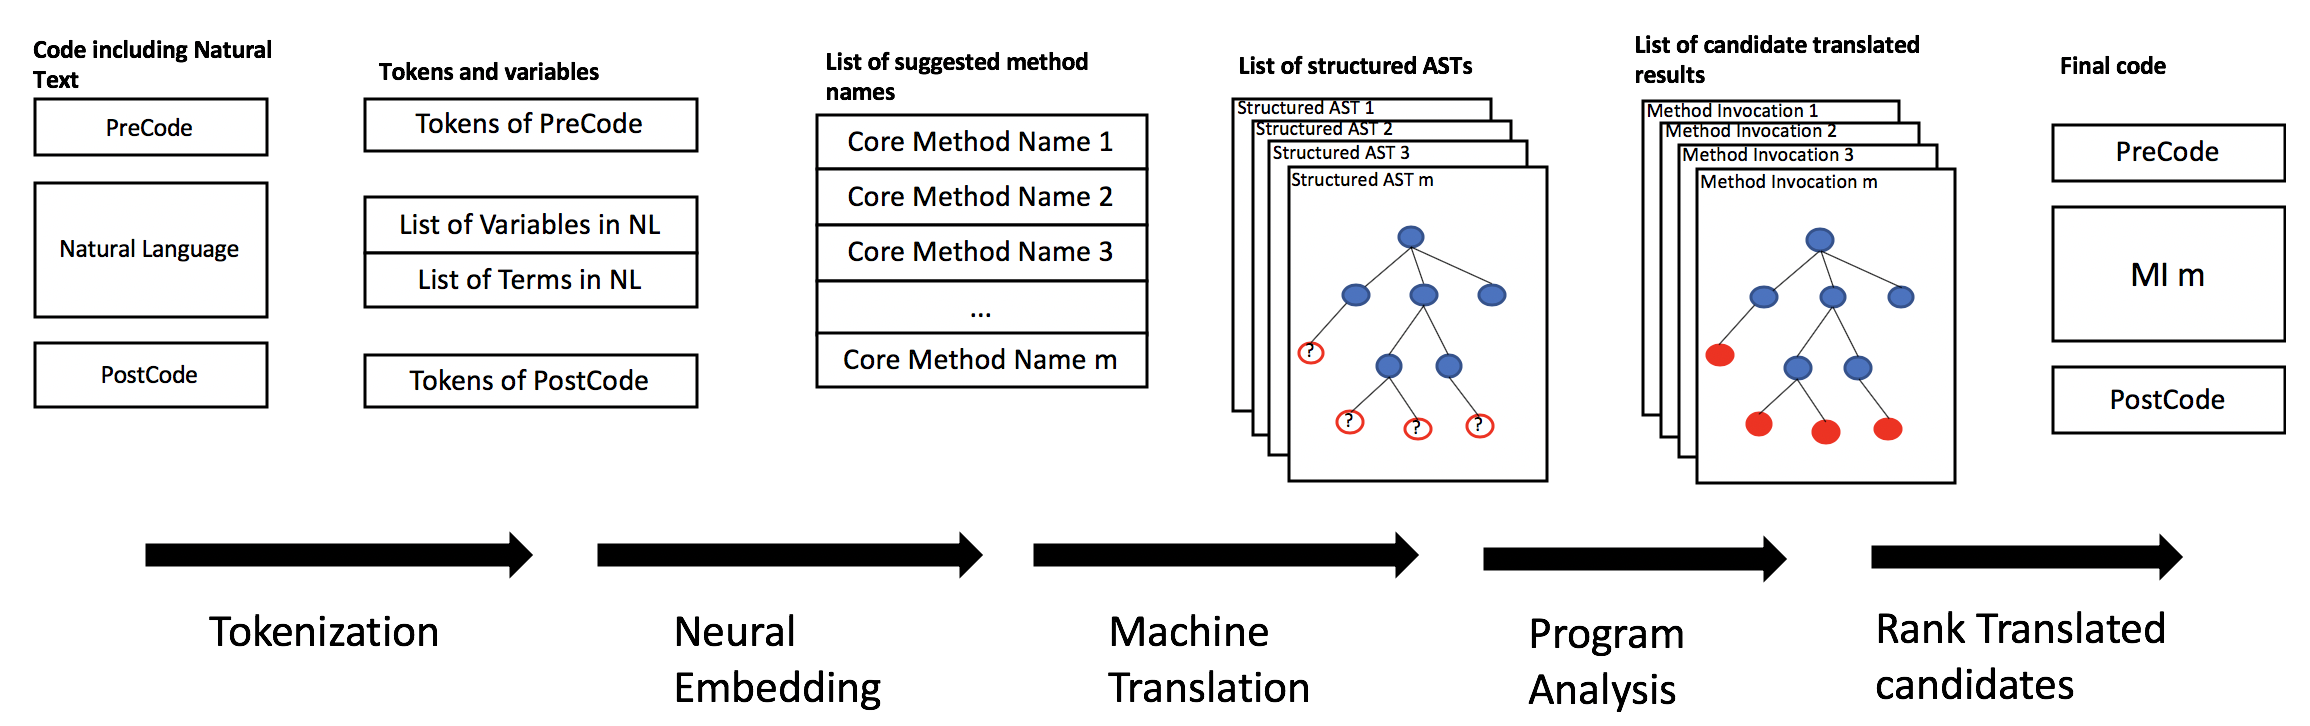
\includegraphics[width=\linewidth]
        {images/InvocMapOverview.png}}
        \caption{Overview of InvocMap model}
        \label{figOverview} 
\end{figure}
\begin{figure}
        \center{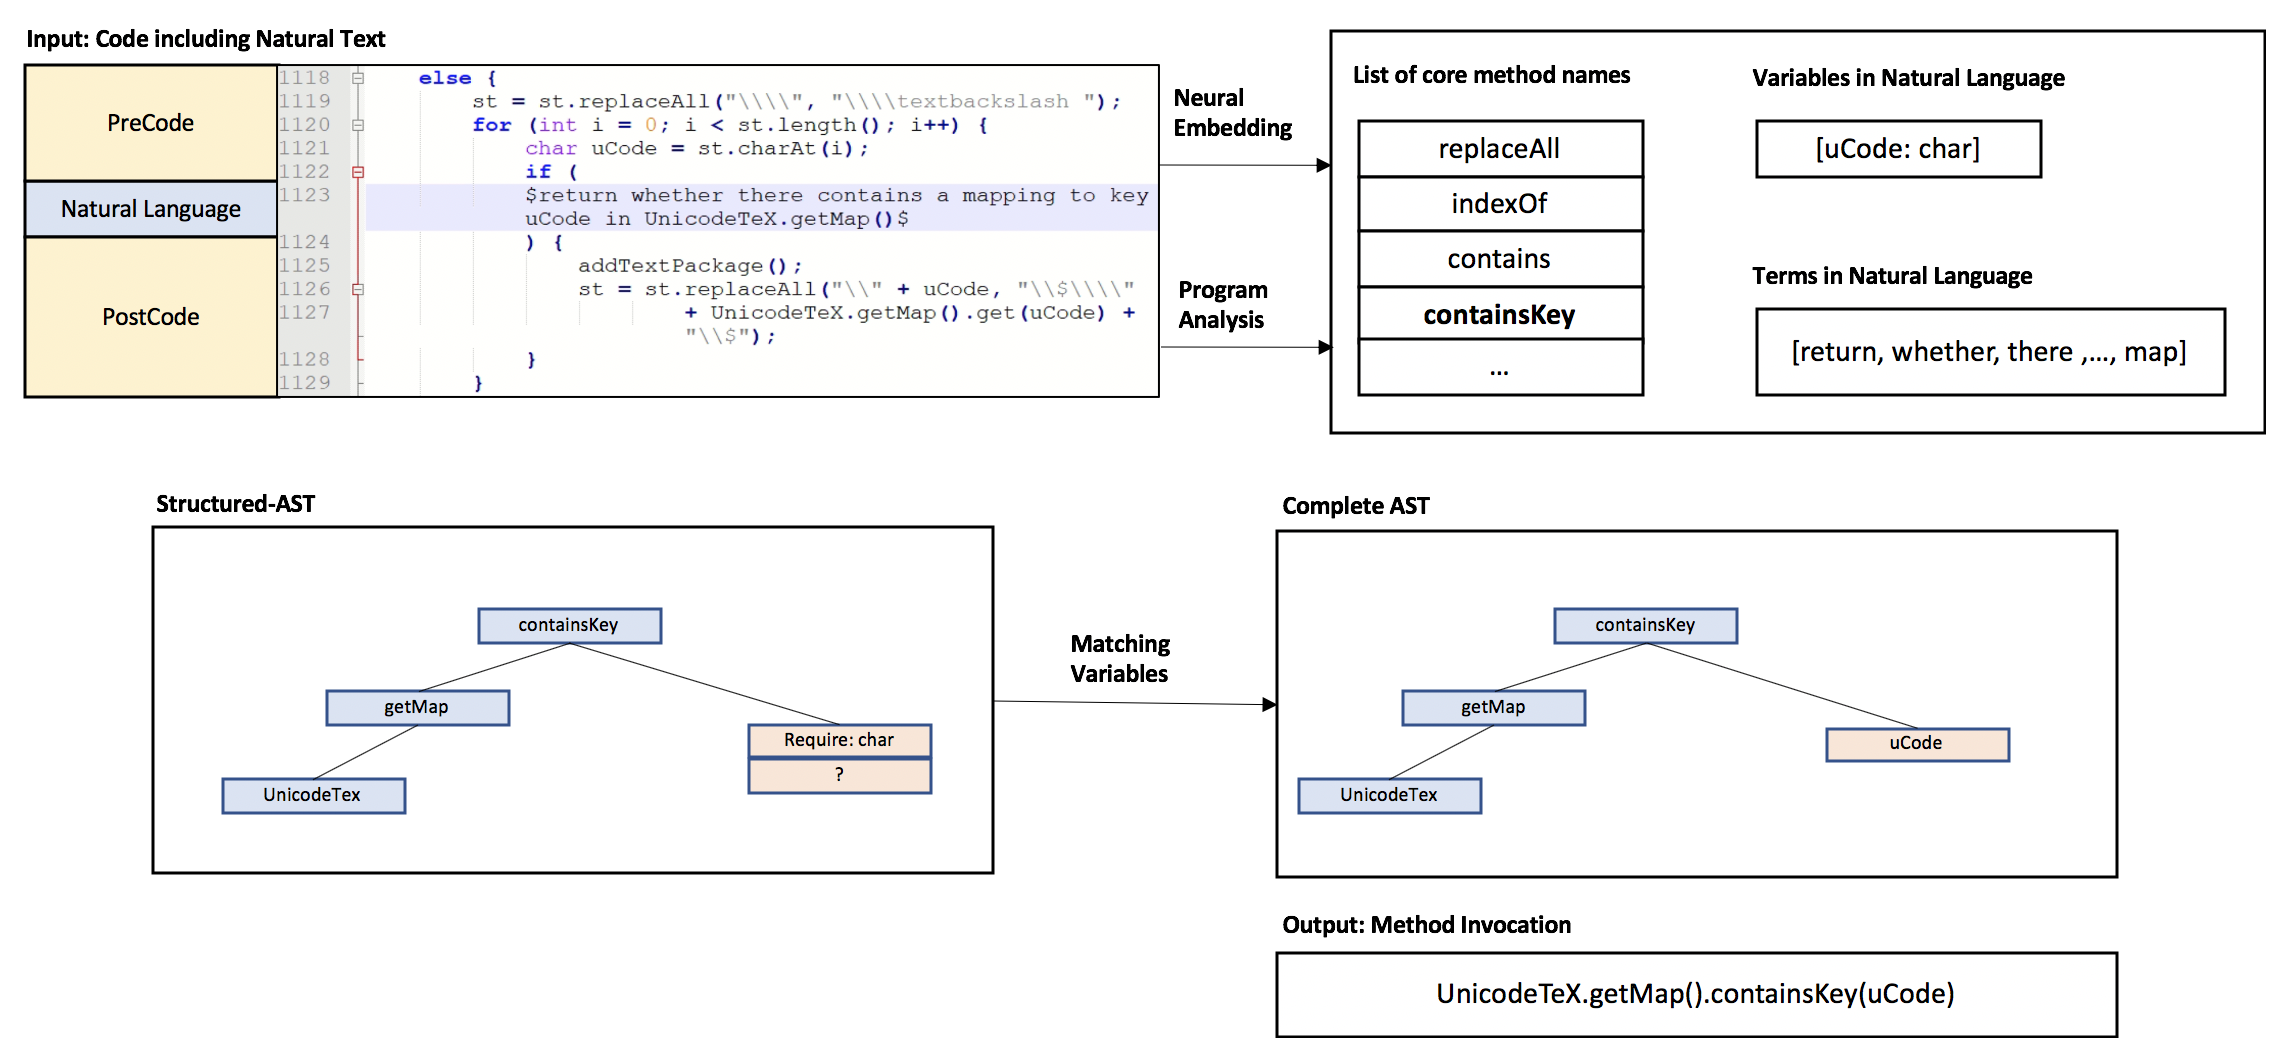
\includegraphics[width=\linewidth]
        {images/MotivatingExample.png}}
        \caption{Motivating Example of InvocMap}
        \label{figMotivatingExample} 
\end{figure}
\subsection{Code and Natural Language tokenization}
For NL-E, InvocMap extract 3 types of information: C-MN, terms and variables. Tokenization provides information about terms and variables. There are two types of variables we detect from NL-E, literals and normal identifier. For literals, we consider string wrapped by quote character as string literal and words that can be converted to number as Integer or Double literal. For identifiers, we provide Program Analysis (PA) module to extract all variables of PreCode of NL-E. The set of variables in PreCode will be compared with each tokens in NL-E to output the variables of NL-E. Other tokens which didn't appear in that set will be as terms of NL.
\\
For Code, we extract all tokens related to PreCode and PostCode of LP-CS. In  Software Engineering (SE), the vocabulary of code elements are larger compared to NLP \cite{013}, which hinders the performance of Machine Learning models. To alleviate this problem, we only represent PreCode and PostCode by their partial types instead of their unique names from code data set. In the other words, if there are 2 variables of PreCode that have the same type, their representation by tokenization will be the same.

\subsection{Neural Embedding based for core method name inference}
While information about terms and variables of NL-E can be extracted by PA, the information about C-MN is hidden from the view point of developers. Based on our study on the NL corpus as queries of AnyCode \cite{007}, we see that though many of NL queries contain words that appeared in C-MN, there is no heuristic rules to extract C-MN from NL queries. To overcome this task, we apply a Neural Embedding solution using Doc2Vec \cite{002}.

Doc2Vec solves the C-MN inference problem by Neural Embedding as the extension of well-known word vectorization Word2Vec \cite{014}. Both Word2Vec relies on the idea of training the vector representation for words/ sentences by 2 types of problem. The first problem is Continuous Bag Of Words (CBOW), which predicts the next tokens from the list of previous tokens. The second problem is Skip Gram model, which learned the representation of surrounding tokens given the current tokens. The most popular model of Doc2Vec defined in \cite{002} relies on CBOW, called Distributed Memory version of Paragraph Vector (PV-DM).
\\
The original Word2Vec stores information of words' vector by a matrix W, which each column represents vector of a word in the vocabulary. Doc2Vec manages words in the same matrix but it add one more matrix which stores the data for each paragraph by a column in a paragraph matrix D. In our problem, given a sequence of code tokens for PreCode as $tok_{1},...,tok_{m}$, the prediction of $tok_{m}$ given previous sequence is computed by Equation \ref{eq:D2VPredict}. In this equation, $y_{i}$ is called un-normalized log-probability for each token $i$, calculated by Equation \ref{eq:D2VLogProbability}. U,b are softmax parameters while h is a function which combines vectors of words and sequence of tokens. \texttt{k} is the size of context surrounding the current token.

\begin{equation} 
\label{eq:D2VPredict}
 p(tok_{m}|tok_{m-k},...,tok_{m+k})=\frac{e^{y_{tok_{m}}}}{\sum _{i} e^{y_{i}}}
\end{equation}
\begin{equation} 
\label{eq:D2VLogProbability}
 y=b+U*h(tok_{m-k},...,tok_{m+k};W;D)
\end{equation}

% \begin{LTXexample}[style=ListingSample,caption={Algorithm for C-MN inference from NL element},label={algmNeuralEmbedding}]
% \begin{lstlisting}[language=Octave,caption={Algorithm for C-MN inference from NL element},label={algmNeuralEmbedding}]  
% Input:
%     Literate Programming Code C;
%     List of method contexts in training set M[];
%     Size of list of suggested method names k;
% Output: 
%     List of method names O;

% %prepare models by training data
% preModel <- trainDoc2VecByPreCodeTokens(M)
% postModel <- trainDoc2VecByPostCodeTokens(M)

% %get list of suggested method names from precode and postcode
% preMethods <-getClosestMethods(C,preModel,k)
% postMethods <-getClosestMethods(C,postModel,k)

% %combine 2 list of suggestions
% O <-combineAndFilter(preMethods,postMethods)


% \end{lstlisting}

\begin{algorithm}
    \caption{Algorithm for C-MN inference from NL element}\label{algmNeuralEmbedding}
    \hspace*{\algorithmicindent} \textbf{Input:}
     Literate Programming Code C;
    List of method contexts in training set M[];
    Size of list of suggested method names k;
    \\
    \hspace*{\algorithmicindent} \textbf{Output:} 
    List of method names O;
    \begin{algorithmic}[1]
    \Procedure{getSuggestedMethodNamesFromNaturalInput}{}
%    \Procedure{MyProcedure}{$x,y$}
%     % Input:
%     \Comment{Input: x}
%     % Output:
%     \Comment{Output:y}

    \State $\textit{preModel} \gets \textit{trainDoc2VecByPreCodeTokens(M)} $
    \Comment{prepare models by training data}
    \State $\textit{postModel} \gets \textit{trainDoc2VecByPostCodeTokens(M)} $
    \\
    \State $\textit{preMethods} \gets \textit{getClosestMethods(C,preModel,k)} $
    \Comment{get list of suggested method names}
    \State $\textit{postMethods} \gets \textit{getClosestMethods(C,postModel,k)} $
    \\
    \State $\textit{O} \gets \textit{combineAndFilter(preMethods,postMethods)} $
    \Comment{combine 2 lists of suggestions}
    
    \EndProcedure
    \end{algorithmic}
    \end{algorithm}

We use Doc2Vec to train the PreCode and PostCode sequences for all method names appeared in our training data set. It provides 2 models which represents all code sequences before and after C-MNs. For a given LP-CS, we extract vectors for PreCode and PostCode of LP-CS. Next, we get the list of method names which have closest representation in 2 contexts of information in LP-CS. Final, the list of C-MNs of PreCode and PostCode are combined. To get best performance, we restrict the size of suggested list to 100 for both lists of PreCode and PostCode. Details of this module is shown in Algorithm \ref{algmNeuralEmbedding}.

\subsection{Mapping Structured ASTs from core method names}
From our knowledge, Statistical Machine Translation (SMT) \cite{015} and Neural Machine Translation \cite{019} are two well-known approaches for translation in Natural Language Processing (NLP). We ran the NMT model by our data and retrieve lower result than SMT model, due to the fact that code data set has large vocabulary which already pointed out in another research \cite{013}. To learn the mapping between C-MN to S-AST, we apply the SMT (\cite{015}). SMT was built from two models: the language model and the translation model. 

Language Model (LM) plays an important role in a PBMT system. LM is used to predict the next token given a sequence of tokens (\cite{016}). The more comprehensive corpus of target language do we have, the LM model quality for prediction is higher.  In our problem, we use the n-gram language model with 4-grams, which was proposed in (\cite{017}). Our n-gram LM is used to measure the probability of the next S-AST given a list of previous implementations. Assume that we have m tokens in the target language \({SAST_{1},...,SAST_{m}}\), the probability provided by LM is:

\begin{equation} 
\label{eq:EQ_Probability}
 P_{LM}[SAST_{1}, ...,SAST_{m}]=\prod_{i=1}^{m}P[SAST_{i} | SAST_{i-n},...,SAST_{i-1}]
\end{equation}
\\

The translation model calculates the probability of a phrase from source language that can be translated to a phrase in a target language. In our problem, if we have a sentence   \({D}\) as the translated result of sentence \({S}\) as tokens in the source language, the selection of \({D}\) as the best candidate is calculated by Equation \ref{eq:EQ_Argmax}. In this equation, \({p(S|D)}\) is the probability of translation model to get the best accuracy calculated in \cite{016}.
\begin{equation} 
\label{eq:EQ_Argmax}
 D_{best}=argmax_{D}(p(S|D)*P_{LM}(D)))
\end{equation}


\subsection{Assigning variables to Structured AST}
The output of MT for each LP-CS is the list of S-AST which missed information of local variables. This module is used to instrumented these missing information. The list of variables in NL-E and a given S-AST are input of the algorithm. For each nodes that don't have variables (i.e red nodes in S-AST Figure \ref{figMotivatingExample}), they will be checked if they match with one of variables in NL-E. The data of S-AST provides the types of missing variables, which helps the algorithm to compare with information in NL-E.
\subsection{Ranking translated candidates }
This module sorts the list of translated MIs based on their completeness in both viewpoints of Natural Language and Programming Language. We provide a heuristic approach which works as the combination of 4 scores. They are \textbf{ScoreMatchOfSAST, ScoreVarsNLE,  ScoreTermsNLE, ScoreComplexityOfSAST}. \textbf{ScoreMatchOfSAST }and \textbf{ScoreComplexityOfAST} penalize MIs with missing nodes and simple structure. \textbf{ScoreVarsNLE} penalizes MIs if there are variables in NL-E that couldn't match into them. \textbf{ScoreTermsNLE} penalize MIs which cannot have many terms in NLE. The total score for raking is shown in Equation \ref{eq:RankTransCandidates}. We fixed 4 parameters \textbf{$\alpha  , \beta , \gamma , \delta $} as \textbf{$0.6, 0.2, 0.1, 0.1$} respectively.

% \begin{equation} 
% \label{eq:RankTransCandidates}
\begin{align}
 Score(MI) &= \alpha*ScoreVarsNLE(MI) + \beta*ScoreMatchOfSAST(MI) \nonumber\\ &\qquad +\gamma*ScoreComplexityOfSAST(MI) + \delta*ScoreTermsNLE(MI) \label{eq:RankTransCandidates}
\end{align}
% \end{equation}

\section{Evaluation}
\ref{tbl:datasetOverview} \\
We evaluate the advantages of InvocMap against state-of-the-art method and analyze the accuracy of each modules. We conduct following research questions:
\begin{enumerate}[\indent {}]
        \item \textbf{Q1}  How developers need for code suggestion from Method Name and from Natural Language?
        \item \textbf{Q2} What is the accuracy of Neural Embedding for suggesting core method names  from natural language and surrounding code?
        \item \textbf{Q3} What is the accuracy of Machine Translation model for inferring structured AST from C-MNs?
        \item \textbf{Q4} What is the accuracy of InvocMap model for inferring code for realizing Literate Programming?
\end{enumerate}

\subsection{Data Preparation}
We provide an automatic approach for collecting high quality Java projects for our evaluation. However, with evaluation data set which are Literate Programming Code Snippets, we need to conduct manually. AnyCode (\cite{007}) provided a data set of 45 NL queries and their related code. However we cannot use this data set for several reasons. First, AnyCode uses the corpus of Github projects from 2013, which some popular software libraries in this corpus are outdated such as \texttt{java.awt} (now it is usually replaced by \texttt{javax.swing}). Second, these queries is suitable for MI search which doesn't consider the surrounding code. We also notice that many expected MIs in this data set doesn't appear in well-known Q&A forums such as StackOverflow \cite{021} and ProgramCreek \cite{020}. We contact the author of AnyCode \cite{007} and see that the tool and the data of this work are not available anymore. Important statistics on our data set is shown in Table \ref{tbl:datasetOverview}.
\\

\textbf{Preparing Training Data} We collect 1000 highest stars Java projects that contain MIs in 6 popular Java libraries: \texttt{GWT}, \texttt{JodaTime}, \texttt{Java Development Kit (JDK)}, \texttt{android}, \texttt{Hibernate} and \texttt{Xstream}. We inherit these criterion for selecting Java projects from another SE engineering research on type suggestion from incomplete code snippet \cite{022}. From this corpus, we extract a parallel corpus, which contains each entity as pairs of list of C-MNs in the source language and list of S-ASTs in the target language. The source side corpus is used in training Neural Embedding module for C-MNs suggestion. Each entity in the corpus represents all information of a method body in 1000 projects. In total, we extract over 800000 pairs for parallel corpus and over 1.77 millions context of C-MNs.
\\
For the configuration, we apply MT toolkit Phrasal \cite{015} with the default configuration. The default mode has number of n-gram as 7-grams and beam size for candidate searching as 100.For Neural Embedding, we use default Neural Network configuration of the Python library \texttt{gensim.Doc2Vec} \cite{023}. We train MT module and Neural Embedding module both on a high end computer with core-i7 processor, 32GB of RAM and RTX 2080 8GB as graphic card.
\\
\textbf{Preparing data set of LP-CSs} We extract this data set by following steps. First, we select randomly a subset of 100 code snippets from the training data set. Then we hire 6 senior students in Bachelor of Computer Science to replace information of MIs to natural language elements. Next, they create natural language elements (NL-Es) for each code snippets and double check with each other to have agreements on each NL-Es. We end up with 100 NL-Es embedded in 100 LP-CSs for evaluation.  






\begin{table}[]
\caption{Data Set Overview}
\label{tbl:datasetOverview}
\centering
\begin{tabular}{|l|r|}
\hline
\multicolumn{1}{|c|}{\textbf{Item}}                & \multicolumn{1}{c|}{\textbf{Number}} \\ \hline
Java projects                                      & 1000                                 \\ \hline
Size of Neural Embedding (NE) corpus               & 1770000                              \\ \hline
Size of Machine Translation corpus                 & 800000                                                               \\ \hline
Number of developers conduct data set of LP-CS        & 6                                    \\ \hline
Size of LP-CSs & 100                                  \\ \hline
Number of developers conduct in study of Q1        & 2                                    \\ \hline
Number of code snippet with NL in Q1               & 40                                   \\ \hline
\end{tabular}
\end{table}
\subsection{Baseline Method}
In the performance comparison, we compare InvocMap with state-of-the-art PCFG based expression synthesization tool AnyCode.
\\
\textbf{AnyCode} \cite{007}: We use the accracy reported as top-1 accuracy by their experiment on 45 NL free-form query. The accuracy of prior work is shown in Table \ref{tbl:Q4ResultAccuracy}. 
\subsection{Performance Evaluation}
To answer \textbf{Q1}, we ask 2 software engineers with more than 7 years of programming experiences in Java to conduct a study. In this study, we ask them to manually getting the expressions of 20 LP-CSs, then we compare between their prediction and expected results which can be in one of three levels. The \texttt{Cannot} level means that the prediction from developers are totally different to the expected output. The \texttt{SomeParts} means the prediction contains some similar nodes to the expected MI. The \texttt{AllParts} means the prediction is totally matched with the expected MI. Since we support for getting MIs by 2 modes: C-MN and NL-E, we conduct two modes of input to developers. The result is shown in Figure \ref{tbl:StudyQ1}. This result shows that developers seems to predict the code better if they know the C-MN of MIs at 55\% of totally correct. With NL-E, things are more difficult since only 40\% of questions have the correct result. This result supports our two assumptions. First, information of C-MN is important which can be solved as the core input for translation. Second, the NL-E to MI inference problem is much more challenging, due to the natural of NL which can contain ambiguous.

\begin{table}[]
\caption{Result on study Q1}
\label{tbl:StudyQ1}
\centering
\begin{tabular}{|l|r|r|r|}
\hline
\multicolumn{1}{|c|}{\textbf{Input}} & \multicolumn{1}{l|}{\textbf{Cannot}} & \multicolumn{1}{l|}{\textbf{SomeParts}} & \multicolumn{1}{l|}{\textbf{AllParts}} \\ \hline
Core Method Name                     & 10\%                                 & 35\%                                    & 55\%                                   \\ \hline
Natural Language                     & 40\%                                 & 20\%                                    & 40\%                                   \\ \hline
\end{tabular}
\end{table}

The \textbf{Q2} question answers how good of an important model performs in InvocMap. In this experiment, we analyze the performance of Doc2Vec for C-MN suggestion using PreCode, PostCode and combination between PreCode and PostCode of 100 LP-CSs. The result shows that the combination of both context achieves the best accuracy at 93\%. We notice that if the NL-E placed at the beginning of the code snippet, the PostCode provides more important roles for the prediction and vice versa.
\\
We answer \textbf{Q3} by the evaluation of our MT engine. We variate the source language from containing only information about C-MNs, information of C-MNs along with their local variables and information of C-MNs, variables in some terms inside MIs. We evaluate on over 1.7 millions C-MNs in our data set by 10 folds cross validation. We got the highest precision at 89.33\% and F1 as 84.4\% shown in Table \ref{tbl:Q3Result}. This shows the power of MT in tokens to S-AST tree generation. The lower of F1 score compared to precision score is due to out of vocabulary problems, which some MIs appeared only less than 10 times in the corpus. The problem of vocabulary matched with the observation of other research work \cite{013}.
\\
The \textbf{Q4} shows us the benefit of InvocMap for realizing LP. We compare the expected MI to the list of suggested MIs by well-known similarity metric called Leveinstein distance \cite{024}. From the result shown in Table \ref{tbl:Q4ResultAccuracy}, we see that InvocMap outperforms AnyCode, which shows the advantages of embedding infotmation of surrounding context with PreCode and PostCode of NL-E for MIs' generation. We achieved 61\% of accuracy, which is remarkably higher accuracy than AnyCode \cite{007}. The accuracy improves to 70\% in top-5 accuracy as shown in Table \ref{tbl:Q4ResultTopK}.
\\
\textbf{Result Analysis} We look at each translated results to investigate possible disadvantages for future works. From this 100 LP-CSs, there are 31 to 37 cases that produced the translated result actually the same with the expected results as shown in Table \ref{tbl:Q4ResultExactMatch}. Examples of these cases are cases \textit{33, 42, 2} of Table \ref{tbl:Q4StudyResult}. From these cases, we notice that the C-MNs are usually not mentioned by exact words, which causes simple textual similarity approach failed to achieve the correct C-MNs. For example, in case \texttt{44}, the word \texttt{"establish"} has the same meaning with \texttt{"get"}. In case \texttt{33}, the phrase \texttt{"square root"} mapped to \texttt{sqrt}, which is expensive if we detect the mapping only by simple rules. In these cases, the surrounding code context provides advantages to infer the correct C-MN. For cases of not entirely matching between translated result and expected result, we analyze some observations that helps us to improve our work.
\\
\textbf{The translated result has same functionality to the expected one}. There are two types of this mismatch. First, as shown in case \texttt{80}, the order of 2 arguments changed in the translated result. Second, the translated result provides string representation of the object like \texttt{20}. In this case, developers need to modify the translated result with one remove action of method name to get the expected one. We can improve this work by checking if the return type of MI matched with the surrounding context to correct the MI.
\\
\textbf{Ambiguities in NL} Currently we use a simple strategy for detecting variables appeared in NL by textual matching. A drawback of this solution is shown in case \texttt{68} of Table \ref{tbl:Q4StudyResult}. In this case, the term \texttt{"color"} is incorrectly mapped as a variable in NL-E, which causes incorrect translated result which requires to map this incorrect variable to its S-AST. We investigate this case and see that the output expression is actually solved as the initialization of variable \texttt{color} in the code. We can improve this disadvantage by restricting the set of variables in source code by its relation to MIs of NL-E.  


\begin{table}[]
\caption{Result of NL-E to C-MN inference by Neural Embedding}
\label{tbl:Q2Result}
\centering
\begin{tabular}{|l|l|l|l|}
\hline
\textbf{} & \textbf{PreCode}          & \textbf{PostCode}         & \textbf{Combine}          \\ \hline
Acccuracy & \multicolumn{1}{r|}{76\%} & \multicolumn{1}{r|}{76\%} & \multicolumn{1}{r|}{93\%} \\ \hline
\end{tabular}
\end{table}



\begin{table}[]

\caption{Result of C-MN to S-AST inference by MT}
\label{tbl:Q3Result}

\centering
\begin{tabular}{|l|r|r|r|}
\hline
\multicolumn{1}{|c|}{\textbf{Types of Evaluation}} & \multicolumn{3}{c|}{\textbf{Cross Validation}}                                                                                             \\ \hline
\multicolumn{1}{|c|}{\textbf{Metric}}              & \multicolumn{1}{c|}{\textbf{Precision}} & \multicolumn{1}{c|}{\textbf{Recall}} & \multicolumn{1}{c|}{\textbf{F1}}  \\ \hline
Core Method Name (C-MN)                            & 70.43\%                                   & 75.89\%                                & 73.06\%                                                        \\ \hline
C-MN and variables                                 & 84.04\%                                   & 78.98\%                                & 81.43\%                                                      \\ \hline
C-MN, variables and terms                          & 89.33\%                                   & 79.98\%                                & 84.4\%                                                            \\ \hline
\end{tabular}
\end{table}


\begin{table}[]
\caption{Result of accuracy for NL-E to MI inference}
\label{tbl:Q4ResultAccuracy}
\centering
\begin{tabular}{|l|r|}
\hline
\multicolumn{1}{|c|}{\textbf{Approach}} & \multicolumn{1}{c|}{\textbf{Accuracy in Top 1}} \\ \hline
AnyCode                                 & 44\%                                            \\ \hline
InvocMap                                & 61.19\%                                         \\ \hline
\end{tabular}
\end{table}

\begin{table}[]
\caption{Result of accuracy of InvocMap from Top-1 to Top-5}
\label{tbl:Q4ResultTopK}
\centering
\begin{tabular}{|l|r|}
\hline
\multicolumn{1}{|c|}{\textbf{Top result}} & \multicolumn{1}{c|}{\textbf{Accuracy}} \\ \hline
Top-1                                     & 61.19\%                                \\ \hline
Top-2                                     & 64.94\%                                \\ \hline
Top-3                                     & 68.13\%                                \\ \hline
Top-4                                     & 69.04\%                                \\ \hline
Top-5                                     & 70.02\%                                \\ \hline
\end{tabular}
\end{table}

\begin{table}[]
\caption{Result of exact match evaluation}
\label{tbl:Q4ResultExactMatch}
\centering
\begin{tabular}{|l|r|}
\hline
\multicolumn{1}{|c|}{\textbf{Top result}} & \multicolumn{1}{c|}{\textbf{Num of exact-match}} \\ \hline
InvocMap Top-1                            & 31                                               \\ \hline
InvocMap Top-10                           & 37                                               \\ \hline
\end{tabular}
\end{table}

\begin{table}[]
\caption{Analysis between expected results and translated results}
\label{tbl:Q4StudyResult}
\centering
\begin{tabular}{|l|l|}
\hline
\multicolumn{1}{|c|}{\textbf{ID}} & \multicolumn{1}{c|}{\textbf{Natural Language / Expected result / Translated result}}        \\ \hline
\multicolumn{1}{|r|}{33}          & return square root of minDelta for Math                                                     \\ \hline
\rowcolor[HTML]{DAE8FC} 
                                  & \cellcolor[HTML]{DAE8FC}                                                                    \\ \cline{1-1}
\rowcolor[HTML]{DAE8FC} 
                                  & \multirow{-2}{*}{\cellcolor[HTML]{DAE8FC}Math.sqrt(minDelta)}                               \\ \hline
\multicolumn{1}{|r|}{44}          & attempt to establish connection to given jdbcUrl DbUser DbPwd for DriverManager             \\ \hline
\rowcolor[HTML]{DAE8FC} 
                                  & \cellcolor[HTML]{DAE8FC}                                                                    \\ \cline{1-1}
\rowcolor[HTML]{DAE8FC} 
                                  & \multirow{-2}{*}{\cellcolor[HTML]{DAE8FC}DriverManager.getConnection(jdbcUrl,DbUser,DbPwd)} \\ \hline
\multicolumn{1}{|r|}{2}           & return whether there contains a mapping to key uCode in UnicodeTeX.getMap()                 \\ \hline
\rowcolor[HTML]{DAE8FC} 
                                  & \cellcolor[HTML]{DAE8FC}                                                                    \\ \cline{1-1}
\rowcolor[HTML]{DAE8FC} 
                                  & \multirow{-2}{*}{\cellcolor[HTML]{DAE8FC}UnicodeTeX.getMap().containsKey(uCode)}            \\ \hline
\multicolumn{1}{|r|}{80}          & return the minimum of lp.height and height                                                  \\ \hline
\rowcolor[HTML]{FFCCC9} 
                                  & Math.min(lp.height,height)                                                                  \\ \hline
\rowcolor[HTML]{FFCCC9} 
                                  & Math.min(height,lp.height)                                                                  \\ \hline
\multicolumn{1}{|r|}{20}          & format now.getTime() into String and append to dateFormatter for SimpleDateFormat           \\ \hline
\rowcolor[HTML]{FFCCC9} 
                                  & dateFormatter.format(now.getTime())                                                         \\ \hline
\rowcolor[HTML]{FFCCC9} 
                                  & dateFormatter.format(now.getTime()).toString()                                              \\ \hline
\multicolumn{1}{|r|}{68}          & return a color from default key "MenuItem.acceleratorForeground" for UIManager              \\ \hline
\rowcolor[HTML]{FFCCC9} 
                                  & UIManager.getColor("MenuItem.acceleratorForeground")                                        \\ \hline
\rowcolor[HTML]{FFCCC9} 
                                  & UIManager.put("MenuItem.acceleratorForeground",color)                                       \\ \hline
\end{tabular}
\end{table}

\section{Related Work}
Although there is no work which realize LP by automatically deriving code for NL with considering surrounding code from our knowledge, research on NL to code is an important research problem in SE. A well-known concept which is related to this problem is called Naturalistic Programming (NP) \cite{024}. NaturalJava \cite{026} is the first tool that realized NP by a heuristic approach to identify important element in NL query to generate fundamental statements in Java. AnyCode \cite{007} is another work followed the idea of NP by constructing a PCFG model for synthesizing MI. We conduct a study of all research works which cited \cite{007} in Google Scholar system and find 54 papers until May, 2020. From these papers, we see that there is no work directly compared their approach with AnyCode. In these works, \cite{028} uses the same input with AnyCode but produces a sequence of Application Programming Interface (APIs) instead of represent them as a tree structure which can be usable in compiler. Some researches works for NL to code with other types of code such as \cite{027,029,030,031,036}. \cite{032,033} use other types of input to generate MI. \cite{034,035} apply the idea of PCFG language model for other research problems. In summary, these 54 papers have different input, different output or focus on different research problems to AnyCode.
\\
There are works that applied Machine Learning for Natural Language to code and vice versa. \cite{009} generates pseudo code from source code by tree to string MT. Our work inherited this idea to provide solution for code generation as inference from C-MN tokens to S-AST trees. \cite{037,010} applies deep learning translation for code generation. The output of \cite{037} is at token level which cannot be used directly in program compiler, while \cite{010} shows the challenge of deriving code by a supervised approach based on noise on practical data. \cite{013} pointed out other problems that hindered Neural Machine Translation in SE research, which is large scale vocabulary.
\section{Conclusion and Future Work}
In this work, we provide InvocMap, a semi-supervised approach for realizing Literate Programming, which handles code snippets as combination of NL-E and surrounding code to generate codes as MIs. The experiment shows our approach outperforms the prior literature AnyCode \cite{007}, proves the potential of our approach. Interesting future works include improving Neural Machine Translation by techniques for solving large vocabolary problems like \cite{013}, implement other vectorization techniques that are suitable for code, extending the Literate Programming support for code fragments instead of expressions, improving the approach by analyzing possible ambiguities in NL-E, and testing our system with larger data set that can have multiple NL-E in the same LP-CS. All of code, data and result of InvocMap are available at \cite{000}.
\clearpage
\bibliography{references}{}
%this may not be right style for nips
\bibliographystyle{plain}


\end{document}
